\documentclass[10pt,a4paper]{article}
\usepackage[utf8]{inputenc}
\usepackage{amsmath}
\usepackage{amsfonts}
\usepackage{amssymb}
\usepackage{graphicx}
\usepackage{enumerate}
\begin{document}

\section{Set Theory}

To demystify mathematics consider
\begin{enumerate}[(i)]
\item What is a theorem?
\item What is a proof?
\end{enumerate}
What if we don't know the answer?

To begin we need
\begin{enumerate}[(a)]
\item an example(s)
\item a nearly related concept
\end{enumerate}


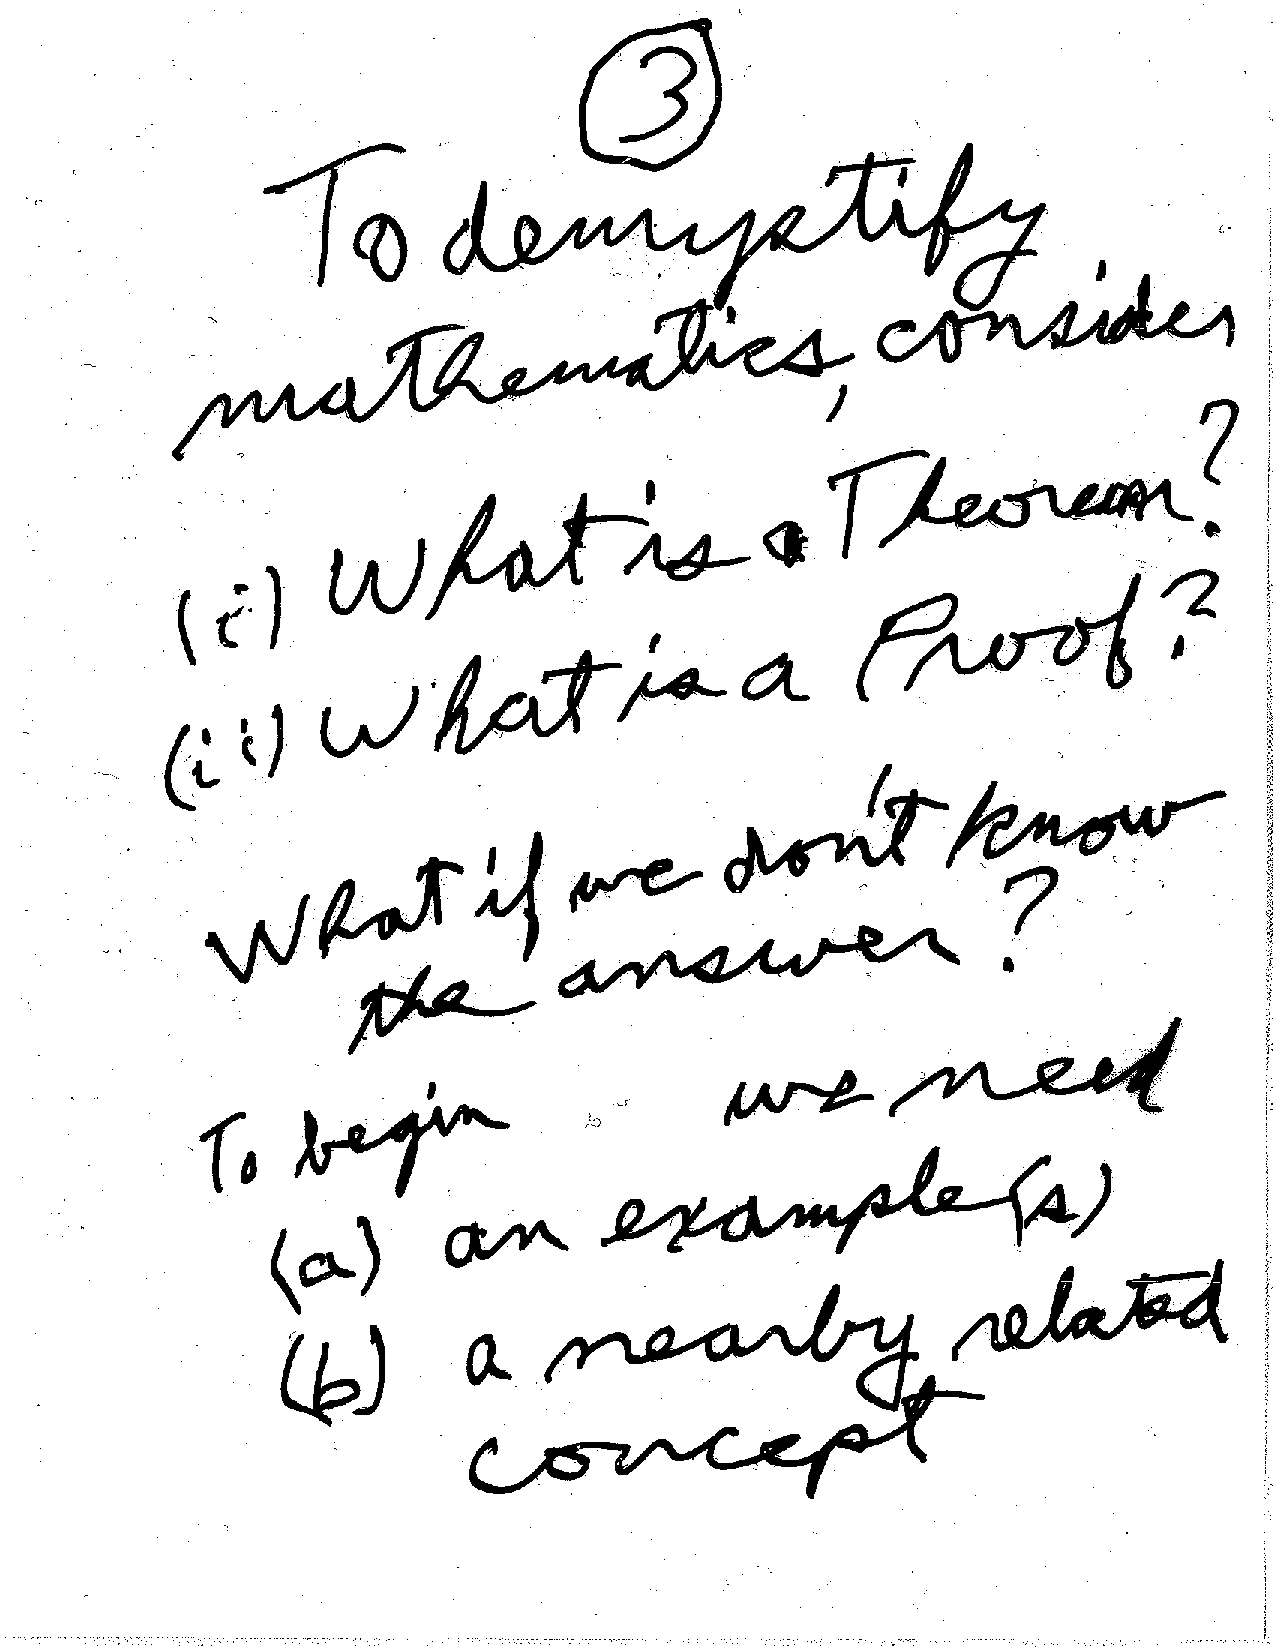
\includegraphics[scale=.5]{Pages/ST_3}

\newpage

Related Concept: Greek Syllogism

\underline{example:}
\begin{enumerate}
\item All men are mortal.
\item Socrates is a man.
\item Therefore, Socrates must die. 
\end{enumerate}

To analyze, recast in set theoretic terms via Venn Diagram.

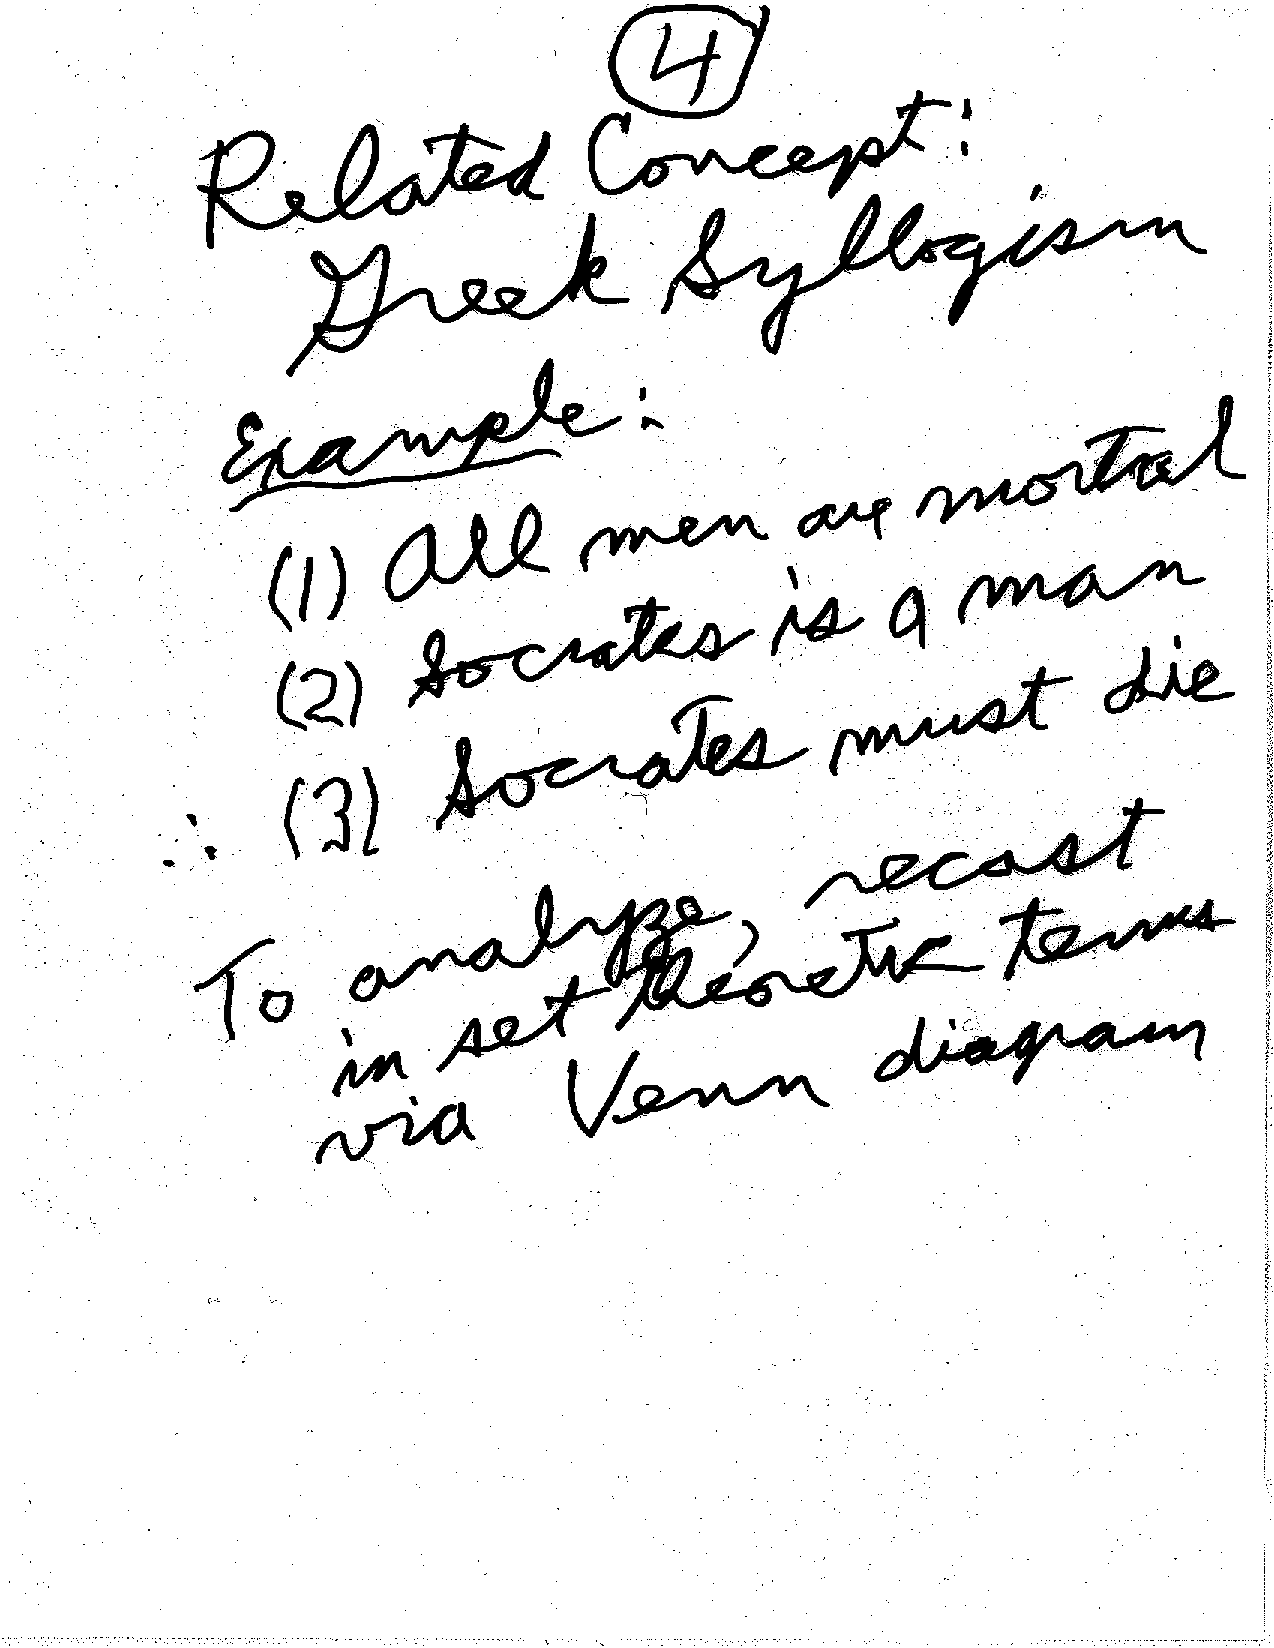
\includegraphics[scale=.5]{Pages/ST_4}

\newpage

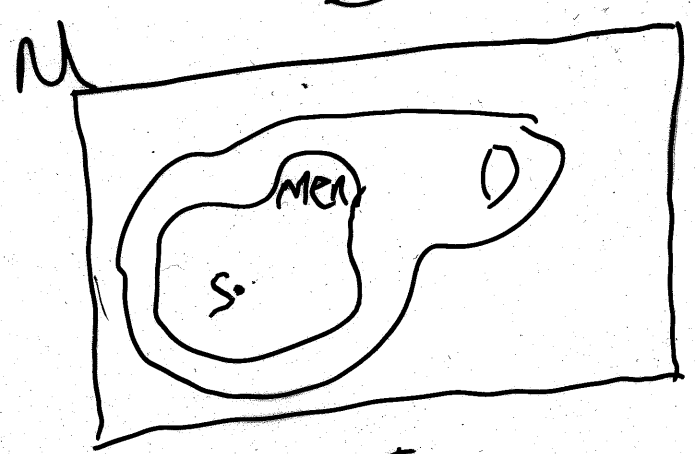
\includegraphics[scale=.2]{Pages/ST_5_im1}

$S$: Socrates\\
$M$: Set of Men\\
$D$: Things that will die\\
$\mathcal{U}$: Things on Earth

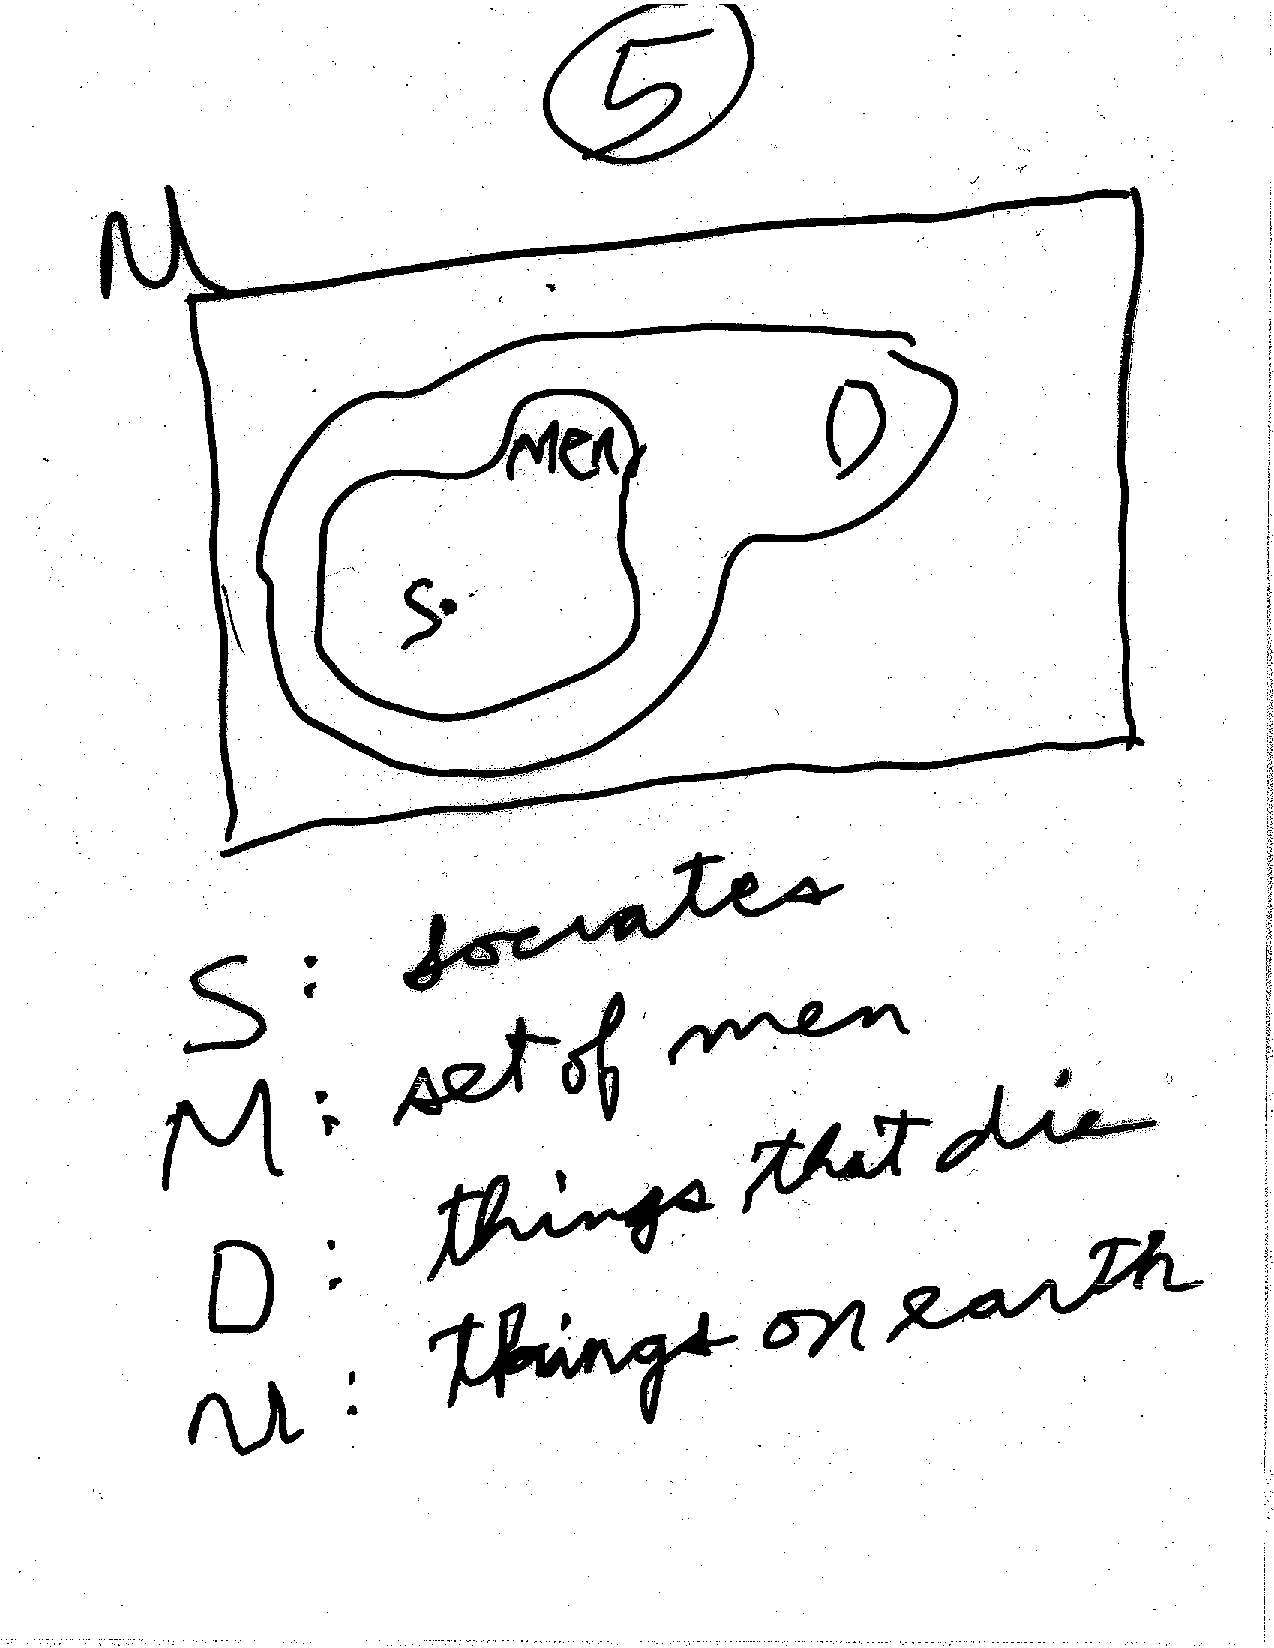
\includegraphics[scale=.5]{Pages/ST_5} 



%Zack: Pages 6,7,8,19,20
\newpage
Notice:
proper noun Socrates 
became an $\frac {element} {(point)}$

common noun \underline{men}
became a \underline{set}
(collection of pts)

\underline{the property} of being mortal became a \underline{set} the universe of all things under consider became the Universe of Possibilities 

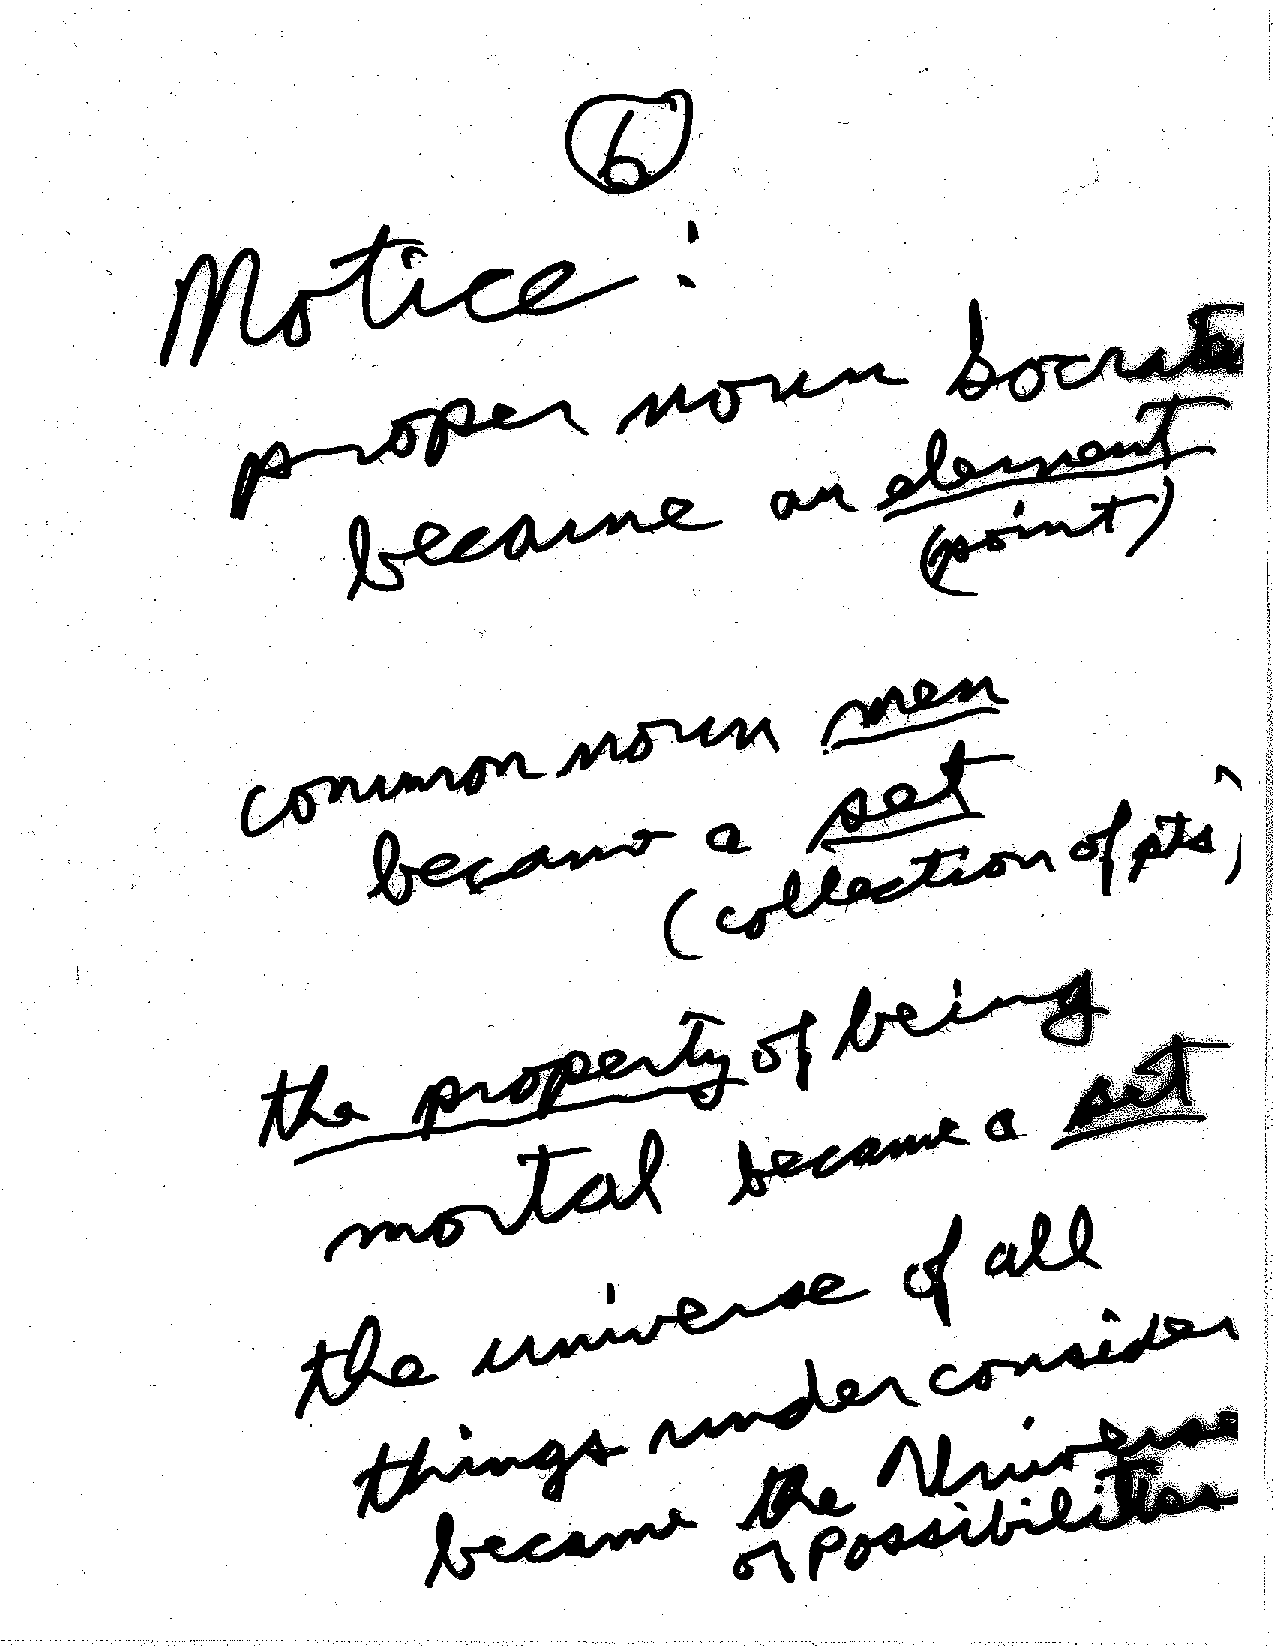
\includegraphics[scale=.5]{Pages/ST_6} 
\newpage
The set theoretic representation of the syllogism:\\
(1)$M\leq D$\\
(2)S$\varepsilon$M\\
(3)S$\varepsilon$D\\
Rearranging, we obtain a more logical ordering of the facts (doing so by successive inclusion):\\ S$\varepsilon$M, $M\leq D$; S$\varepsilon$D\\
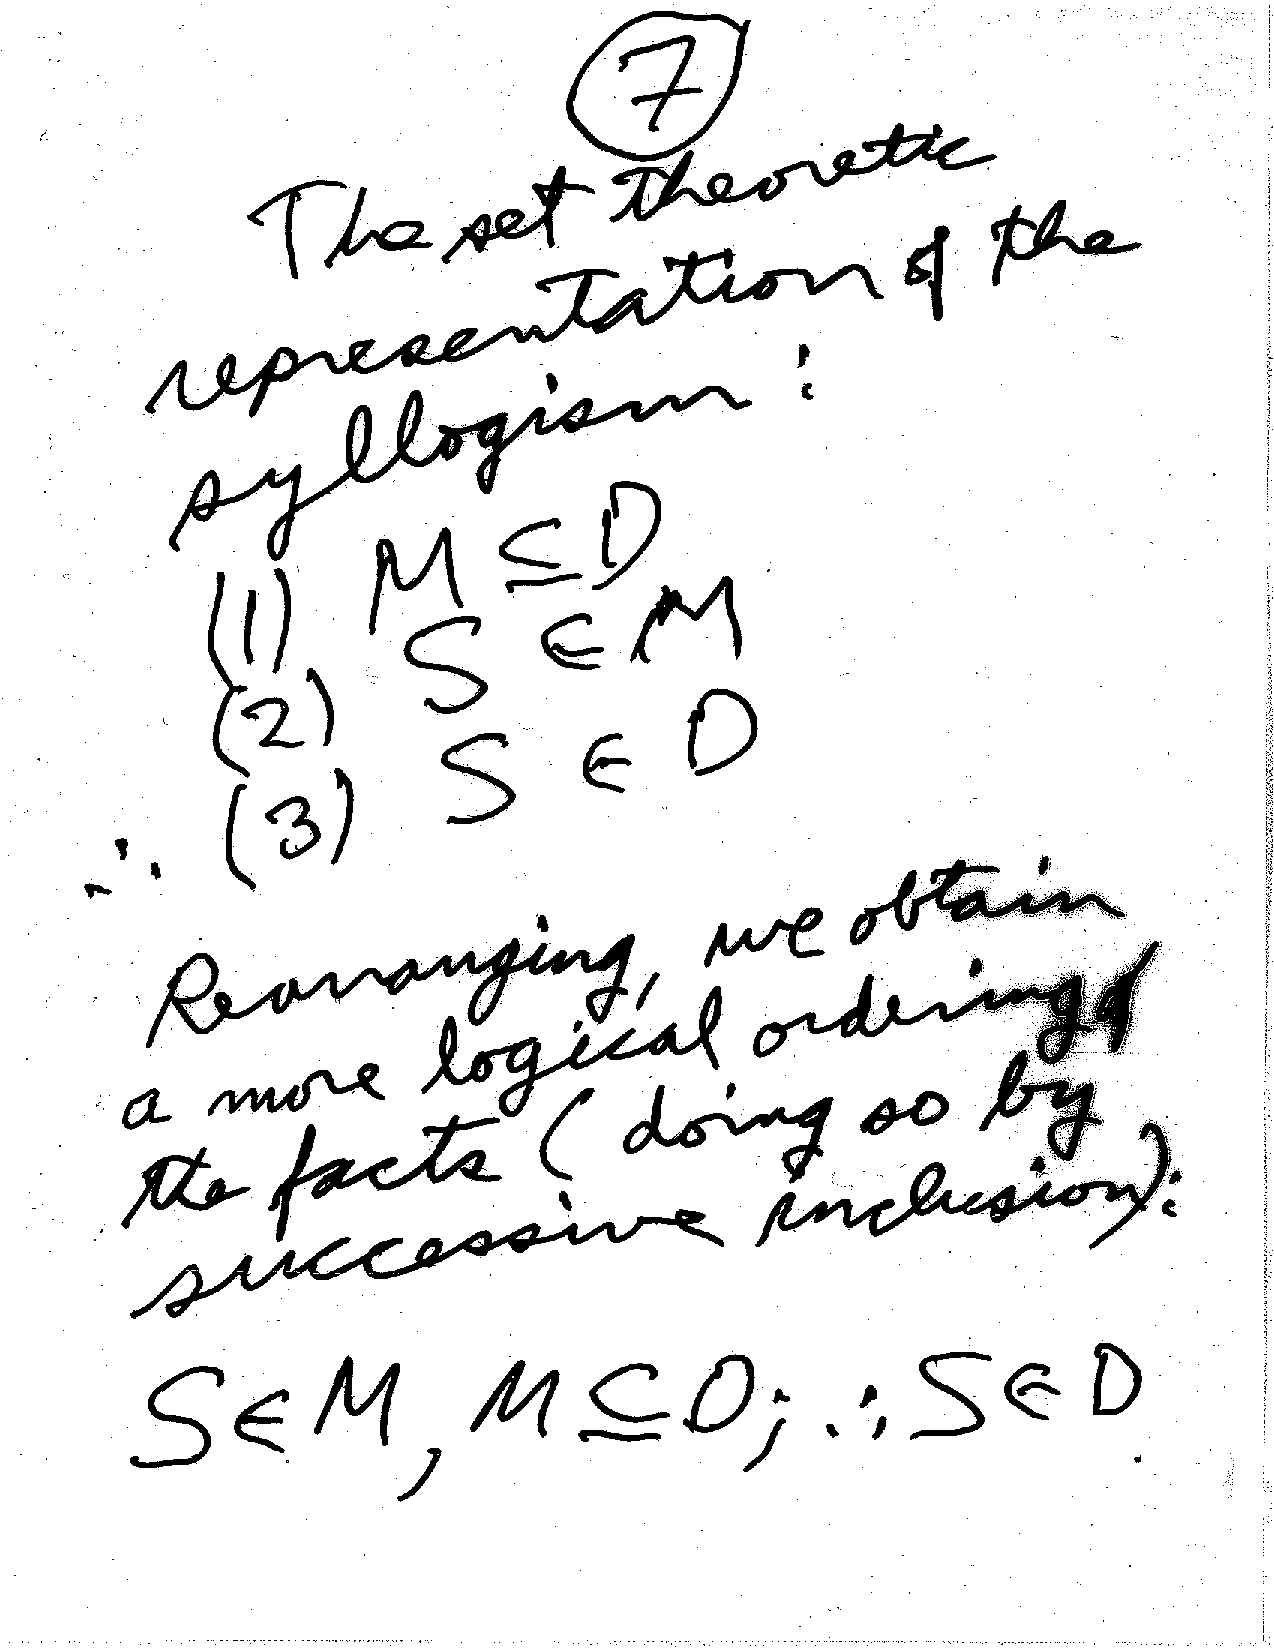
\includegraphics[scale=.5]{Pages/ST_7} 
\newpage
What has the syllogism taught us?
\begin{enumerate}
\item Games of fact (Truth on falsehood) can be put in a set theoretic context.\\
\item The simplest deductive argument has the form if $X\varepsilon$A and $A\leq B$ then $X \varepsilon$ B
\end{enumerate}
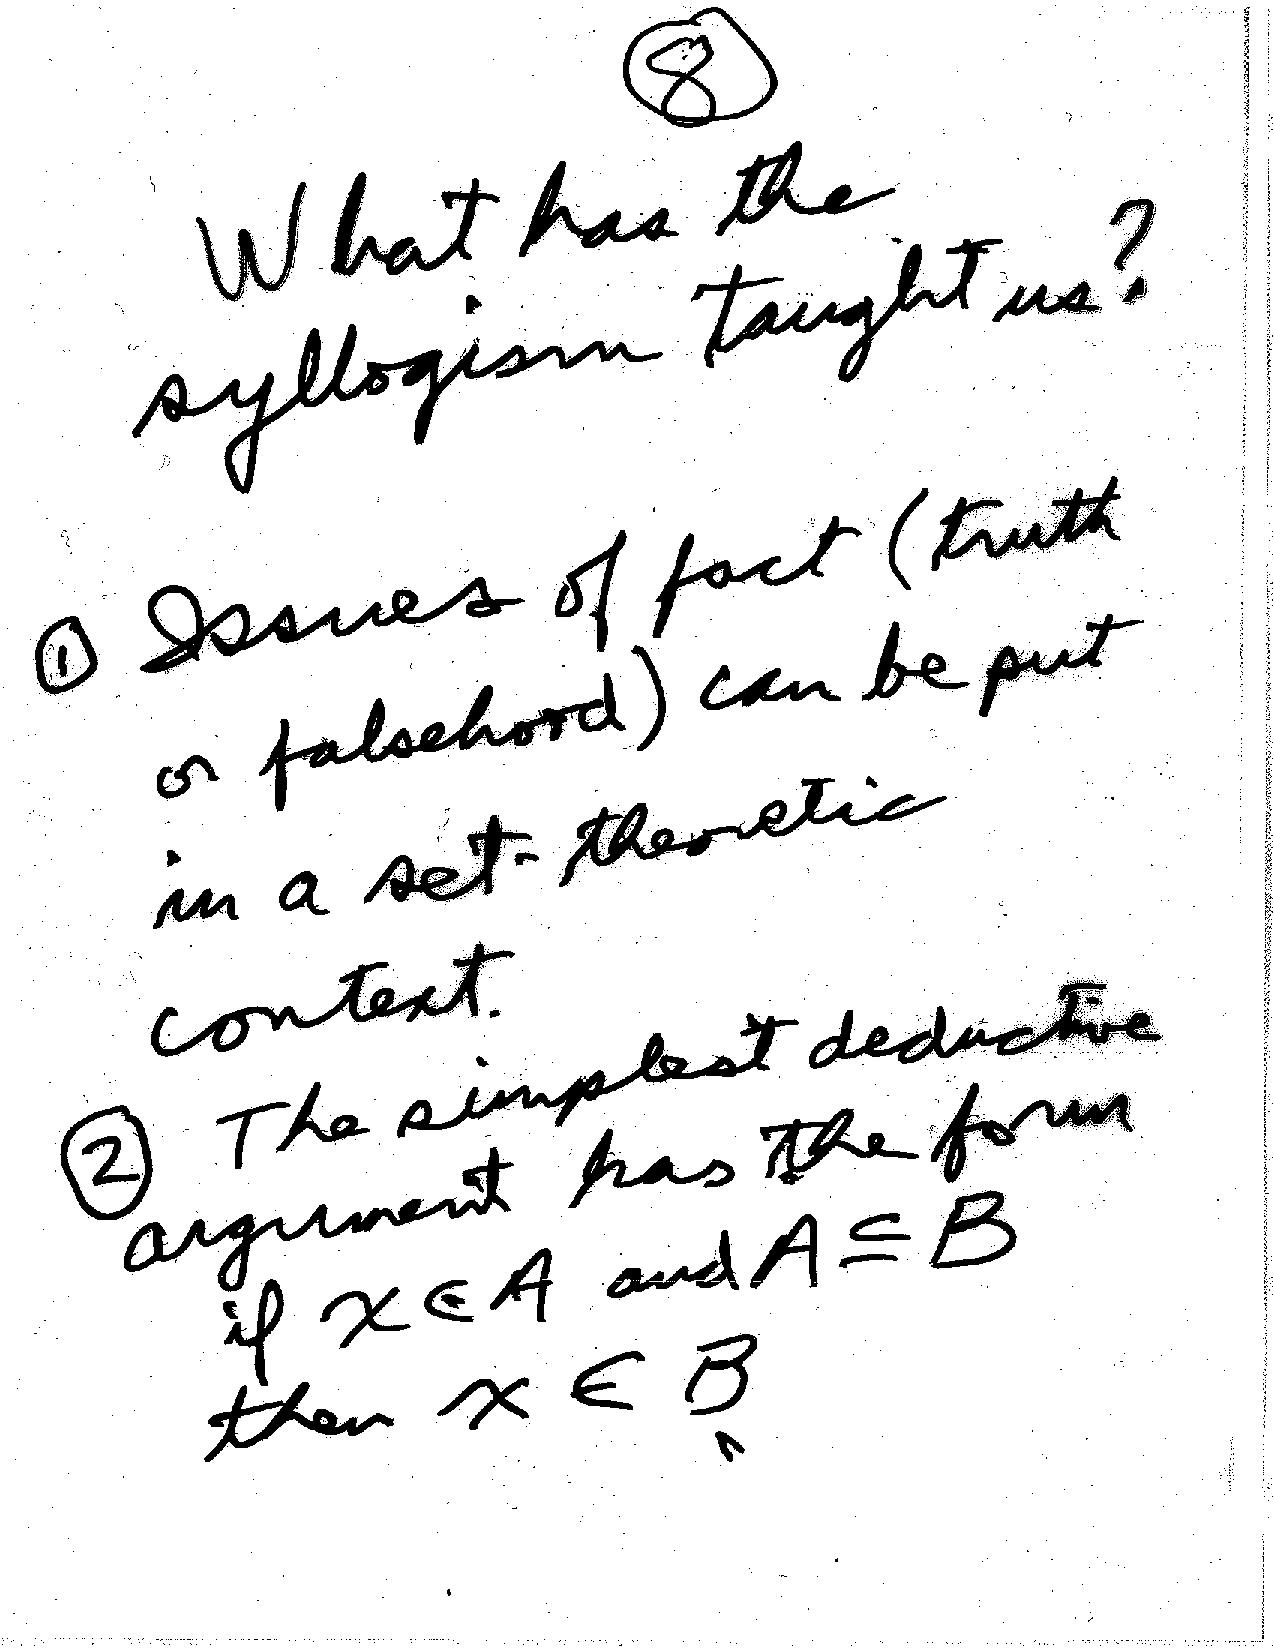
\includegraphics[scale=.5]{Pages/ST_8}


%Jack: 21, 9, 10, 11

%Koka: Pages 13, 13A, 22 ,22A, 22B


\section{Generate $\mathbb{N}$}


%Ruth: Pages L4A-L4G




\section{From $\mathbb{Z}$ to $\mathbb{R}$ via ordering}
%Jazz: ZR1-ZR5

%Kyler: ZR6 - ZR10

%Preethika: ZR11-ZR14


\section{Sequence and Limits}

%Aaron: First 2 pages and 48-50

%Hamza: 51-52B

\section{Limit and Convergence}

%Joe: 50-51

%Quinten: 52-53

%Farishta: 53A-54A

\section{Infinite Series}

%Sukhreet: IS1 - IS 7

%Matthew: IS8 - IS15

%Will: IS16 - IS23

%Rebecca: IS24 - IS32

%Maady: IS33 - IS42

\section{Metric Spaces Part 1}

%Travis: M1 - M5

%Jerome: M6- M10



\section{Metric Spaces Part 2}


%Bryant: M1-M7

%Reshma: M8-M14

%Ethan: M15-M21





\end{document}